\documentclass{standalone}
\usepackage{tikz}
\usepackage{amsmath, amssymb, latexsym}
\DeclareMathOperator{\ReLU}{ReLU}
\newcommand{\KL}{\ensuremath{\mathrm{KL}}}
\newcommand{\Ber}{\ensuremath{\mathrm{Ber}}}
 
\usepackage{tikz}
\usepackage{xcolor}
\definecolor{fc}{HTML}{1E90FF}
\definecolor{h}{HTML}{228B22}
\definecolor{bias}{HTML}{87CEFA}
\definecolor{noise}{HTML}{8B008B}
\definecolor{conv}{HTML}{FFA500}
\definecolor{pool}{HTML}{B22222}
\definecolor{up}{HTML}{B22222}
\definecolor{view}{HTML}{FFFFFF}
\definecolor{bn}{HTML}{FFD700}
\tikzset{fc/.style={black,draw=black,fill=fc,rectangle,minimum height=1cm}}
\tikzset{h/.style={black,draw=black,fill=h,rectangle,minimum height=1cm}}
% \tikzset{bias/.style={black,draw=black,fill=bias,rectangle,minimum height=1cm}}
% \tikzset{noise/.style={black,draw=black,fill=noise,rectangle,minimum height=1cm}}
\tikzset{conv/.style={black,draw=black,fill=conv,rectangle,minimum height=1cm}}
% \tikzset{pool/.style={black,draw=black,fill=pool,rectangle,minimum height=1cm}}
% \tikzset{up/.style={black,draw=black,fill=up,rectangle,minimum height=1cm}}
% \tikzset{view/.style={black,draw=black,fill=view,rectangle,minimum height=1cm}}
\tikzset{bn/.style={black,draw=black,fill=bn,rectangle,minimum height=1cm}}
\tikzset{rcb/.style={draw, fill=bias, minimum height=1cm}}
\tikzset{elu/.style={draw, fill=h, minimum height=1cm}}

\newcommand{\bt}{\mathbf{t}}
\newcommand{\bx}{\mathbf{x}}
\newcommand{\by}{\mathbf{y}}
\newcommand{\bz}{\mathbf{z}}
\newcommand{\eq}{=}




\begin{document}

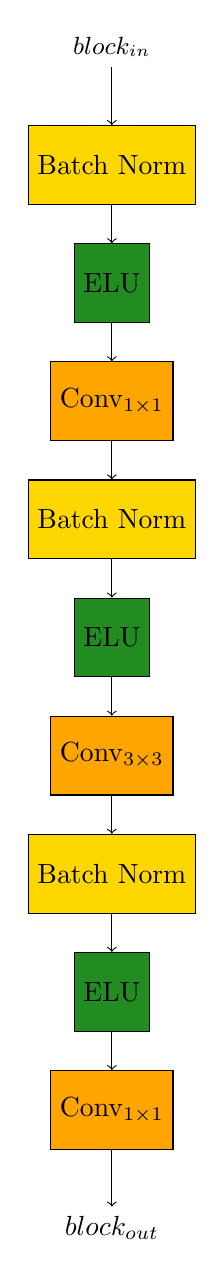
\begin{tikzpicture}
    \node (h) at (0,0) {\small$block_{in}$};
 
    \node[bn] (bn1) at (0, -1.5) {$\text{Batch Norm}$};
    \node[elu] (elu1) at (0, -3) {ELU};
    \node[conv] (conv1) at (0, -4.5) {$\text{Conv}_{1\times1}$};
    
    \node[bn] (bn2) at (0, -6) {$\text{Batch Norm}$};
    \node[elu] (elu2) at (0, -7.5) {ELU};
    \node[conv] (conv2) at (0, -9) {$\text{Conv}_{3\times3}$};
    
    \node[bn] (bn3) at (0, -10.5) {$\text{Batch Norm}$};
    \node[elu] (elu3) at (0, -12) {ELU};
    \node[conv] (conv3) at (0, -13.5) {$\text{Conv}_{1\times1}$};
    
    \node[] (out) at (0, -15) {$block_{out}$};
    
    \draw[->] (h) to (bn1);
    \draw[->] (bn1) to (elu1);
    \draw[->] (elu1) to (conv1);
    
    \draw[->] (conv1) to (bn2);
    \draw[->] (bn2) to (elu2);
    \draw[->] (elu2) to (conv2);
    
    \draw[->] (conv2) to (bn3);
    \draw[->] (bn3) to (elu3);
    \draw[->] (elu3) to (conv3);
    \draw[->] (conv3) to (out);
\end{tikzpicture}
\end{document}